\documentclass{article}
\title{Trying to learn \LaTeX}
\date{\today}
\author{A dumb student}

\usepackage[spanish,es-tabla]{babel}
\usepackage[utf8]{inputenc}
\usepackage{graphicx}
\usepackage{subcaption}

\begin{document}
  \maketitle
  Este es mi primer documento en \LaTeX!
  \[
    \frac{-b \pm \sqrt{b^2 -4ab}}{2a} \\
    \frac{-(2) \pm \sqrt{(2)^2 -4*(-5)*(3)}}{2*(-5)}
  \]

  En este punto vamos a probar que una lista se puede desplegar de este modo
  \begin{itemize}
    \item Go west-Pet Shop Boys
    \item The wolf-Siam\'es
    \item I won't let you down-OK Go
  \end{itemize}

  Ahora bien, lo que haremos es implementar la mítica de una imágen en este lenguage.

  \begin{figure}[h!]
    \centering
    \begin{subfigure}[b]{0.45\linewidth}
      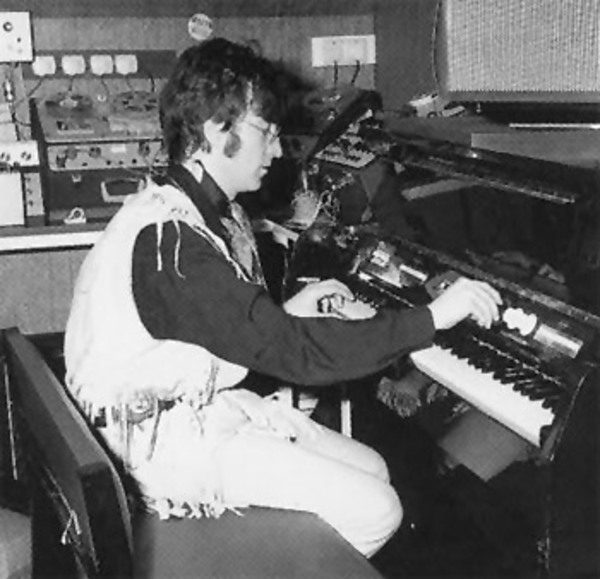
\includegraphics[width=\linewidth]{../../pictures/lennon.jpg}
      \caption{Vista lateral}
      \label{fig:westminster_lateral}
    \end{subfigure}
    \begin{subfigure}[b]{0.45\linewidth}
      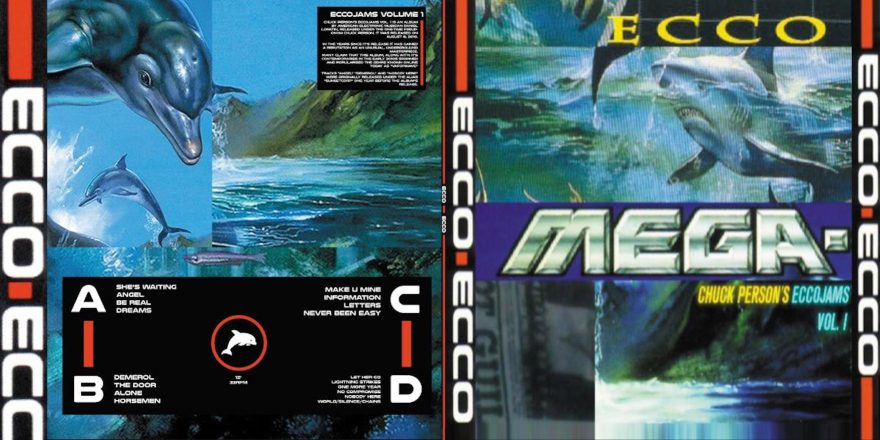
\includegraphics[width=\linewidth]{../../pictures/ecco.jpg}
      \caption{Vista aérea}
      \label{fig:westminster_aerea}
    \end{subfigure}
    \caption{Palacio de Westminster}
    \label{fig:westminster}
  \end{figure}

  Esto es ahora para mostrar una tabla

  \begin{table}[t]
    \begin{center}
      \begin{tabular}{| c | c |}
        \hline
        Fruta & Cantidad \\ \hline
        Manzana & 4 \\
        Naranja & 10 \\
        Plátano & 3 \\ \hline
      \end{tabular}
      \caption{Edta cosa es para la cantidad de frutas}
      \label{tab:prrof}
    \end{center}
  \end{table}
\end{document}
